\documentclass[10pt]{article}

%% Various useful packages and commands from different sources

\usepackage[applemac]{inputenc}
\usepackage[english]{babel}
\usepackage[T1]{fontenc}
\usepackage{cite, url,color} % Citation numbers being automatically sorted and properly "compressed/ranged".
%\usepackage{pgfplots}
\usepackage{graphics,amsfonts}
\usepackage[pdftex]{graphicx}
\usepackage[cmex10]{amsmath}
\usepackage{bm}
% Also, note that the amsmath package sets \interdisplaylinepenalty to 10000
% thus preventing page breaks from occurring within multiline equations. Use:
 \interdisplaylinepenalty=2500
% after loading amsmath to restore such page breaks as IEEEtran.cls normally does.

% Compact lists
\usepackage{enumitem}
\usepackage{booktabs}
\usepackage{fancyvrb}

\usepackage{listings} % for Matlab code
\definecolor{commenti}{rgb}{0.13,0.55,0.13}
\definecolor{stringhe}{rgb}{0.63,0.125,0.94}
\lstloadlanguages{Matlab}
\lstset{% general command to set parameter(s)
framexleftmargin=0mm,
frame=single,
keywordstyle = \color{blue},% blue keywords
identifierstyle =, % nothing happens
commentstyle = \color{commenti}, % comments
stringstyle = \ttfamily \color{stringhe}, % typewriter type for strings
showstringspaces = false, % no special string spaces
emph = {for, if, then, else, end},
emphstyle = \color{blue},
firstnumber = 1,
numbers =right, %  show number_line
numberstyle = \tiny, % style of number_line
stepnumber = 5, % one number_line after stepnumber
numbersep = 5pt,
language = {Matlab},
extendedchars = true,
breaklines = true,
breakautoindent = true,
breakindent = 30pt,
basicstyle=\footnotesize\ttfamily
}

\usepackage{array}
% http://www.ctan.org/tex-archive/macros/latex/required/tools/
\usepackage{mdwmath}
\usepackage{mdwtab}
%mdwtab.sty	-- A complete ground-up rewrite of LaTeX's `tabular' and  `array' environments.  Has lots of advantages over
%		   the standard version, and over the version in `array.sty'.
% *** SUBFIGURE PACKAGES ***
\usepackage[tight,footnotesize]{subfigure}
\usepackage[top=2.2cm, bottom=2.2cm, right=1.7cm,left=1.7cm]{geometry}
\usepackage{indentfirst}


%\setlength\parindent{0pt}
\linespread{1}

\usepackage{mathtools}
\DeclarePairedDelimiter{\ceil}{\lceil}{\rceil}
\DeclarePairedDelimiter{\floor}{\lfloor}{\rfloor}
\DeclareMathOperator*{\argmax}{arg\,max}
\newcommand{\M} {\mathtt{M}}
\newcommand{\dB} {\mathrm{dB}}
\newcommand{\tr} {\mathrm{tr}}
\newcommand{\lmod}[1] {_{\,\mathrm{mod}\,#1}}



\graphicspath{ {figures/} }

% equations are numbered section by section
%\numberwithin{equation}{section}


\begin{document}
\title{Digital Transmission - Homework 3}
\author{Andrea Dittadi, Davide Magrin, Michele Polese}

\maketitle

%%%%%%%%%%%%%%%%%%%%%%%%%%%%%%%%%%%%%%%%%
%%%%%%%%%%%%%% PROBLEM 1 %%%%%%%%%%%%%%%%
%%%%%%%%%%%%%%%%%%%%%%%%%%%%%%%%%%%%%%%%%

\section*{Problem 1}

% Spiegare cosa mandiamo e come lo generiamo
In this problem the channel $q(n\frac{T}{4})$ is given at $T_c = \frac{T}{4}$. The goal is to estimate at the receiver the timing phase $t_0$ and the equivalent channel impulse response in $T$ with LS method.
The setting of the system is as in Fig.~\ref{fig:channel_T4}. In order to perform LS estimation the first $L + N_{seq} = 15 + 10$ symbols of the sequence $a_k$ are binary symbols out of a QPSK constellation with $\sigma_a^2 = 2$. 
In particular they are $1+j$ and $-1-j$ and map the $+1$ and $-1$ values of a ML sequence of length $L = 15$, partially repeated by $N_{seq}=10$. Then QPSK data follows. 
The conversion between a bit stream and QPSK is carried out by the \texttt{bitmap} function. %% TODO some more on this?? Give a better formulation

\begin{figure}
	\centering
	\includegraphics[width = 0.8\textwidth]{channel_T4}
	\caption{System setting for problem 1}
	\label{fig:channel_T4}
\end{figure}

%%TODO Does Eq go in dB???? 

% Spiegare che channel_output funziona da polifase
The noisy output $r_n$ of the channel is computed with a polyphase version of the channel impulse response $q(nT_c)$. Each branch is $q^{i}(mT) = q(mT + i)$ with $i \in [0, 3]$ , and since it is not time-varying it is possible to directly compute the convolution of each branch and the $a_k$ sequence. At the output of each convolution white noise $w_n$ is added, with variance $\sigma_w^2 = \frac{\sigma_a^2 E_q}{4 \Gamma} = -19.2411$ dB, where $\sigma_a^2 = 2$, $E_q = 2.3819$ and $\Gamma = 20$ dB is the given SNR at receiver input. Then a parallel to series converter generates the output at time $T_c$.

% !!! Spiegare come stimiamo t0, riportare l'equazione (Formula 7.269, channel_estimator)
The first operation which the receiver does is estimating $t_0$ as optimal timing phase in $T_c$. In particular, given the stream of symbols $r_n$, and the knowledge of the ML sequence $a_l, l\in [0, L-1]$, the receiver computes

\begin{equation}
	m_{opt} = \argmax_m | x_{ra}(mT_c) | = \argmax_{m} | \frac{1}{L} \sum_{l = 0}^{L - 1} x(lT + mT_c)a^* (l) |
\end{equation}
for $ 0 < m < 40$ and finds that
\begin{equation}
	m_{opt} = 10
\end{equation}
\begin{equation}
	t_{0} = m_{opt}T_c = 10 T_c
\end{equation}

Remember that $t_0 = 10$ in $T_c$ and the corresponding $D_{ch} = ({t_0}\lmod{4})T = 2T$ represents the number of samples after which the receiver receives the first sample of the training sequence multiplied by $h_0$, which is the coefficient of the channel impulse response with the greatest amplitude, plus some ISI in the case in which there are some precursors. In other words, if the receiver and the transmitter use the same time index $k$ and if $x_k$ is the output at time $T$ of the receiver then
\begin{equation}
x_{k} = h_0a_{k-D_{ch}} + i_k, \quad i_k = \sum_{\substack{i = -N_1 \\ i \neq 0}}^{N_2} h_i a_{k-D_{ch}-i}
\end{equation}
where $i_k$ is the inter-symbol interference. Therefore, if $t_0 = 10T_c$ and $D_{ch} = 2T$ there could be at most 2 precursors (i.e. the coefficients of $h_i$ for $i = -N_1, \dots, -1$), and they can be equal to 0 (they don't introduce ISI but just the delay $D_{ch}$) or different from 0 but with an amplitude lower than $h_0$. 

The receiver can now perform the estimate of the channel impulse response at time $T$. The output of the channel $r_n$ is sampled at $n = t_0 + kT$ to get $x_k = r_{t_0 + kT}$. The LS estimate is computed using the symbols of the known sent ML sequence $a_k$ and a suitable section of the output. Note that the training sequence sent of length $L + N_{seq} = 25$ has $N_{seq} = 10$ which is enough to avoid the transient of the channel which is $N - 1$, with $N = N_1 + N_2 + 1$ the real length of the impulse response.
Note also that the LS method can estimate a causal impulse response, $\tilde{h}_j, j = 0, \dots, N$, while the channel impulse response could have some precursors which are different from 0, and therefore an anticausal component. In order to correctly estimate $h_i, i = -N_1, \dots, N_2$, given a supposed length $\hat{N} = \hat{N}_1 + \hat{N}_2 + 1$, LS considers $a_k, k = 0, \dots, L+\hat{N}-1$ and the output $x_k, k = D_{ch} - N_1, \dots, D_{ch} - N_1 + L + \hat{N} - 1$ and it performs the estimation in the standard way. This is the same as considering a causal impulse response, with $\hat{N}$ coefficients, but since we suppose that $N_1$ assumes a given value in $0, D_{ch}$, then it is possible to shift the estimate left of $N_1$ samples and obtain the estimate for $\hat{h}_i, i = -N_1, N_2$. 
The actual estimation is performed as in~\cite[p.~246]{bc}, i.e. using a $L \times \hat{N}$ observation matrix

\begin{equation}
	\boldsymbol{\mathcal{I}} =
 \begin{bmatrix}
  a(\hat{N}-1) & \cdots & a(0) \\
  \vdots  & \ddots & \vdots  \\
a[(\hat{N}-1)+(L-1)] & \cdots & a(L-1) \\
 \end{bmatrix}
\end{equation}
and a desired sample vector
\begin{equation}
\mathbf{o}^T = \left[ x(\hat{N}-1)\;,\; \ldots\; , \;x((\hat{N}-1)+(L-1)) \right].
\end{equation}
Therefore we can solve the LS problem as
\begin{equation}
	\hat{\mathbf{h}}= \mathbf{\Phi}^{-1} \boldsymbol{\vartheta}, \quad\mathrm{ with } \quad \mathbf{\Phi}=\boldsymbol{\mathcal{I}}^H \boldsymbol{\mathcal{I}} \quad \mathrm{ and }\quad \boldsymbol{\vartheta} = \boldsymbol{\mathcal{I}}^H \mathbf{o}.
\end{equation}

In particular, in order to estimate as first the length $\hat{N} = N_1 + N_2 + 1$ of the impulse response and $N_1, N_2$, we operate as follows. Let $N_{max} = N_{seq} = 10$ the maximum possible length $\hat{N}$ of the impulse response. As first, we set $N_1 = 0$ and compute the functional of the error 
\begin{equation} 
	\mathcal{E} = \frac{1}{L}\sum_{k = \hat{N} - 1}^{(L-1)+(\hat{N}-1)}|d(k)-\hat{d}(k)|^2
	\label{eq:functional}
\end{equation}
for $N_2 = 0, 1, \dots, N_{max} - N_1 - 1$. This procedure is repeated for $N_1 = 1$ and $2$. The functionals $\mathcal{E}$ for different $N_1$ are then plotted together, against $N_2$, in Fig.~\ref{fig:functional}.
\begin{figure}[h!]
	\centering
	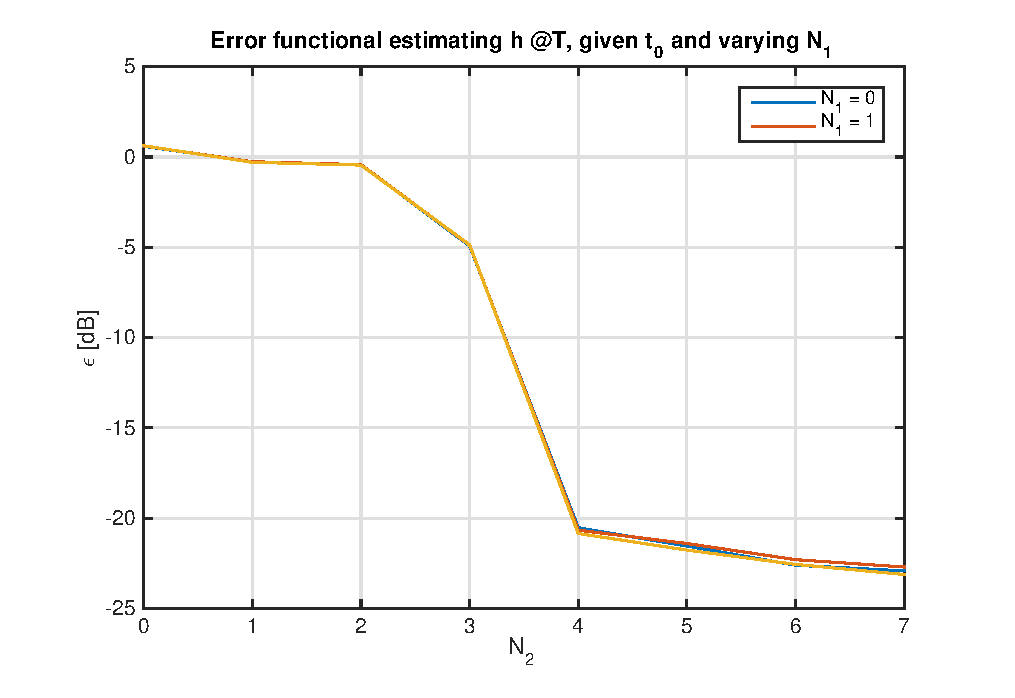
\includegraphics[width = 0.8\textwidth]{error_func_p1}
	\caption{$\mathcal{E}$ vs $N_2$ for different $N_1$}
	\label{fig:functional}
\end{figure}
It can be seen that there's a knee for $N_2 = 4 \forall N_1$, therefore we pick $N_2 = 4$. Then $N_1$ that minimizes $\mathcal{E}$ should be chosen, therefore $N_1 = 2$. However the 3 curves are very close to each other, and choosing $N_1 = 0$ would bring a similar functional $\mathcal{E}$ but a much lower complexity for Viterbi and FBA in the second problem. 

In Tables~\ref{table:h0} and~\ref{table:h2} are reported the amplitude and phase of $h_i, i = -N_1, \dots, N_2$, while in Fig.~\ref{fig:hi_p1} is reported the amplitude of both the choice $N_1 = 0$ and $N_1 = 2$. Note that they are very similar.


% !!! Riportare valori di {h_i_hat} in una tabella, ampiezza e fase
\begin{table}[h!]
	\centering
	\begin{tabular}{c|c|c|c|c|c}
		$i \in [-N_1, N_2]$ & 0 & 1 & 2 & 3 & 4 \\ \hline
		$|h_i|$ 		& 0.7140  &  0.2463  &  0.1553  &  0.5778  &  0.4001 \\
		$\angle(h_i)$ 	& -2.5815  &  1.3137  & -2.5666  & -1.5096  & -1.6715 \\
	\end{tabular}
	\caption{Amplitude and phase of $h_i, i \in [-N_1, N_2]$, for the choice $N_1 = 0$}
	\label{table:h0}
\end{table}

\begin{table}[h!]
	\centering
	\begin{tabular}{c|c|c|c|c|c|c|c}
		$i \in [-N_1, N_2]$ & -2 & -1 & 0 & 1 & 2 & 3 & 4 \\ \hline
		$|h_i|$ 	&	0.0121  &  0.0137  &  0.7136   & 0.2446  &  0.1551  &  0.5853  &  0.4068 \\
		$\angle(h_i)$ &	0.3575  & -2.0494  & -2.5692   & 1.3064  & -2.5498  & -1.5017  & -1.6574 \\
	\end{tabular}
	\caption{Amplitude and phase of $h_i, i \in [-N_1, N_2]$, for the choice $N_1 = 2$}
	\label{table:h2}
\end{table}

% !!! Plottare {h_i_hat} per i = -N_1, ..., N_2
\begin{figure}[h!]
 \centering
 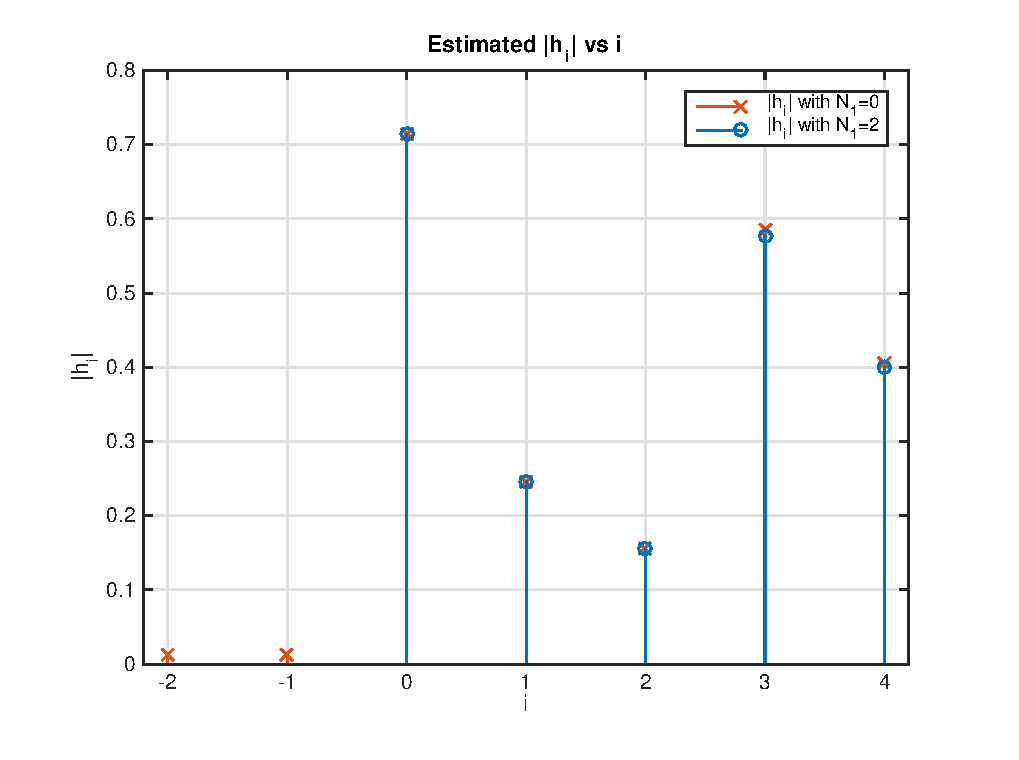
\includegraphics[width = 0.9\textwidth]{hi_p1}
 \caption{$|h_i|, i \in [-N_1, N_2]$ for $N_1 = 0$ and $N_1 = 2$}
 \label{fig:hi_p1}
\end{figure}

% !!! Determinare la stima della varianza del rumore, sigma_w_hat_squared, compararla con sigma_w_squared in dB.
The noise that the channel introduces is $\sigma_w^2 = -19.2411$ dB, while the noise estimate is lower: $\hat{\sigma}_w^2 = -20.5327$ dB for the choice $N_1 = 0$, and $\hat{\sigma}_w^2 = -20.851$ for the choice $N_1 = 2$ (see Eq.~\ref{eq:functional}). Note that this is the value given by a single estimate and not an expectation. However, this shows that a sequence of the given length $L = 15$ is too short to correctly estimate the real noise of the channel, since it averages on a number of noise samples which is close to the length of the impulse response we are trying to estimate. Indeed, by using a longer ML sequence (say 127) the estimate obtained is much closer to the real value also in each single realization. 

% !!! Comparare la stima di Lambda_n_hat con il valore "vero" di Lambda_n_hat, fare le considerazioni su LS per cui il Lambda_n teorico raddoppia quando si usano i simboli ±1±j al posto di ±1.
At last, it is necessary to make some considerations on the fact that the sequence used in this problem is a binary mapping in a QPSK constellation with $\sigma_a^2 = 2$ of a PN sequence. In particular let $a_l = (1+j) p_l$ with $p_l = \pm 1$ a symbol of the PN sequence. Then the autocorrelation of the sequence, of periodicity L, is
\begin{equation}
	r_a(n) = \frac{1}{L}\sum_{l = 0}^{L-1} a_l a^*_{l-n} = \\
	\frac{1}{L}\sum_{l = 0}^{L-1} (1+j)p_l (1-j)p^*_{l-n} = 
	\frac{2}{L} \sum_{l= 0}^{L-1} p_l p^*_{l-n} = 2 r_p(n) = \sigma_a^2 r_p(n)
\end{equation}
with 
\begin{equation}
	r_p(n) = 
  	\begin{cases}
    1       & \quad \text{if } n =0 \\
    -\frac{1}{L}  & \quad \text{if } n \neq 0 \\
  \end{cases}
\end{equation}
Therefore let $\Phi(i, n) = [\mathbf{\Phi}]_{i, n}$. Then
\begin{equation}
	\Phi(i, n) = (L -1 + N - N + 1)r_a(i-n) = \sigma_a^2 Lr_p(i-n)
\end{equation}
At the same time $\vartheta(n) = \sigma_a^2 Lr_{dp}(n)$ with $\boldsymbol{\vartheta} = [\vartheta(0), \dots, \vartheta(N-1)]$.
Therefore the LS can be solved in the usual way, as previously mentioned, with the equation $\hat{\mathbf{h}}= \mathbf{\Phi}^{-1} \boldsymbol{\vartheta}$ and provides the same soultion that a PN sequence would give. 

As for the signal-to-estimation error ratio, it is possible to procede as in \cite{bc}. Let $\boldsymbol{\vartheta} = \sum_{N-1}^{N-1+L-1} x(k) \mathbf{a}^*(k)$ and $\boldsymbol{\xi} = \sum_{N-1}^{N-1+L-1} w(k) \mathbf{x}^*(k)$ we obtain $\boldsymbol{\vartheta} = \boldsymbol{\Phi}\mathbf{h} + \boldsymbol{\xi}$ and finally $\boldsymbol{\Delta h} = \boldsymbol{\Phi}^{-1} \boldsymbol{\xi}$. 
Let's now consider the energy of this vector. Since $w$ is zero mean, with variance $\sigma_w^2$, then
\begin{equation}
	\mathbf{R}_{\boldsymbol{\xi}} = E[\boldsymbol{\xi}^*\boldsymbol{\xi}^T] = \sigma_w^2 \mathbf{\Phi}^*
\end{equation}
and
\begin{equation}
	\mathbf{R}_{\boldsymbol{\Delta h}} = \sigma_w^2 (\mathbf{\Phi}^*)^{-1}
\end{equation}
Then we need $E[||\mathbf{\Delta h}||^2]$ which is
\begin{equation}
	E[||\mathbf{\Delta h}||^2] = \sigma_w^2 \mbox{tr}[(\mathbf{\Phi}^*)^{-1}]
\end{equation}
Finally, since the definition of signal-to-estimation error ratio is 
\begin{equation}
	\Lambda_n = \frac{\sigma_w^2}{\M_a E[||\mathbf{\Delta h}||^2]}
\end{equation}
with $M_a = \sigma_a^2 + (E[a])^2 \approx \sigma_a^2 = 2$ for $L >> 1$. Then in this specific case
\begin{equation}
	\Lambda_n = \frac{\mbox{tr}[(\mathbf{\Phi})^{-1}]}{\sigma_a^2}
\end{equation}
Since $\mathbf{\Phi}$ has the same form of the $\mathbf{\Phi}$ matrix for a PN sequence, with the exception of a multiplicative factor $\sigma_a^2 = 2$, it is possible to use the same derivation of \cite{bc} in order to compute $\Lambda_n$. Let $\mathbf{1}_{N\times N}$ a matrix with all ones, then
\begin{equation}
	\mathbf{\Phi} = \sigma_a^2 ((L+1)\mathbf{I} - \mathbf{1}_{N\times N})
\end{equation}
and
\begin{equation}
	\mathbf{\Phi}^{-1} = \frac{\sigma_a^2}{L+1} \bigg( \mathbf{I} + \frac{\mathbf{1}_{N\times N}}{L+1-N} \bigg)
\end{equation}
Finally, following \cite{bc}, we obtain
\begin{equation}
	\Lambda_n = \frac{\sigma_a^2}{\sigma_a^2}\frac{(L+1)(L+1-N)}{N(L+2-N)}
	\label{eq:lambdateo}
\end{equation}
getting the same result as for a PN sequence.
Finally, some numerical results are reported in Table~\ref{table:lambda}, both for the choice $N_1 = 2$ given by the minimum of the functional and for $N_1 = 0$ given by the practical considerations mentioned above. 
The first column of Table~\ref{table:lambda} contains the estimated value computed as
\begin{equation}
	\Lambda_n = \frac{\hat{\sigma}_w^2}{\M_a E[||\mathbf{\Delta h}||^2]}
	\label{eq:lambdareal}
\end{equation}
Note that $E[||\mathbf{\Delta h}||^2]$ is computed by assuming the real $h_i$ is known and that the value of Equation~\eqref{eq:lambdareal} is affected by the bad estimate of $\sigma_w^2$ given by the choice of a value of $L$ which doesn't provide a long enough training sequence.

\begin{table}[h!]
	\centering
	\begin{tabular}{c|c|c}
				&	As in Eq.~\eqref{eq:lambdareal} [dB]	& As in Eq.~\eqref{eq:lambdateo} [dB]  \\ \hline
	$N_1 = 2$	&	1.82							& 3.13 \\
	$N_1 = 0$	&	1.87							& 1.66 \\
	\end{tabular}
	\caption{$\Lambda_n$ for $N_1 = 0$ and $N_1 = 2$}
	\label{table:lambda}
\end{table}

\clearpage

%%%%%%%%%%%%%%%%%%%%%%%%%%%%%%%%%%%%%%%%%
%%%%%%%%%%%%%% PROBLEM 2 %%%%%%%%%%%%%%%%
%%%%%%%%%%%%%%%%%%%%%%%%%%%%%%%%%%%%%%%%%

\section*{Problem 2}

% Breve descrizione del sistema in T
In this second problem the system works in T, as in Figure~\ref{fig:channelt}, and as SNR we consider $\Gamma = \frac{\sigma_a^2 E_h}{\sigma_w^2}$. 

\begin{figure}
	\centering
	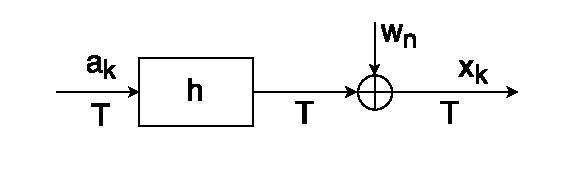
\includegraphics[width=0.6\textwidth]{channel_t}
	\caption{System description for the second problem}
	\label{fig:channelt}
\end{figure}

The output is computed using a sampled version of the provided impulse response $q(nT_c)$ that matches the response estimated in the previous problem, i.e. $h_i = q(iT + m_{opt}), \quad i \in [-N1, N2]$. 

The sequence $a_k$ which is transmitted is composed of a ML binary sequence of 25 symbols, as in Problem 1, which is necessary to perform the channel estimate, and of a QPSK stream of symbols that maps a ML sequence composed of 0s and 1s in order to mimic random transmission of bits. In case more than $2^{20}-1$ bits are needed we partially or completely repeat the longest ML sequence of $2^{20}-1$ bits.

Note that in the following analysis we will consider always the same parameters for the channel, with $N_1 = 0, N_2 = 4$ accordingly to the considerations of Problem 1. However the estimate must be repeated for each different SNR, since the channel noise varies. Moreover, in order to design the system, we consider only the estimated impulse response and not the real one, and since the estimate done with a ML sequence of $L = 15$ is lousy, then also the design will not drive the performance of the receivers as close as possible to the theoretical bound. 

This is computed as in \cite{bc} for the matched filter case (i.e. no ISI) and a QPSK constellation ($M=4$), resulting in 
\begin{equation}
	BER_{MF} = \frac{1}{\log_2 (M)} 4 \bigg(1- \frac{1}{M} \bigg) Q\bigg(\sqrt{\frac{3}{M-1} \Gamma}\bigg) = Q(\sqrt{\Gamma})
	\label{eq:BERmf}
\end{equation}
where $\Gamma$ is the SNR at receiver input, which in the case of a matched filter is equal to $\Gamma = 0.5 M_a \gamma_{MF}= \gamma_{MF}$, with $\gamma_{MF}$ the SNR at detection point for a MF, $M_a = \sigma_a^2$ since the transmitted sequence has 0 mean.

We also computed this bound with a simulation, where the receiver performed a decision over received data with no ISI, $x_k = a_k + w_k$, with $a_k$ a sent symbol, $w_k$ AWGN noise of power $\sigma_w^2 = \sigma_a^2 \ \Gamma$ in order to match the SNR $\Gamma$ of the real channel (which has the $E_h$ factor since the data stream is convolved with the $h_i$ filter). Decision is taken with a threshold detector.

% Considerazioni sull'implementazione di LE e DFE, riportare i grafici di Jmin (qualche grafico), considerazioni su M1, M2, D, riportare i grafici di \hat{h}, c, psi, b per \Gamma = 10 dB
\subsection*{Linear equalizer and Decision Feedback Equalizer}
The simpliest receivers implemented are a linear equalizer (LE) and a decision feedback equalizer (DFE) which try to remove the ISI component from the received samples $x_k$. The decision is then taken with a threshold detector. 

They both use the information known about the channel in order to perform equalization. In particular the LE tries to equalize both the precursors and the postcursors out of the received signal $x_k$, while DFE uses the detected symbols to perform cancellation of the postcursors from a signal already filtered with a feed-forward filter that removes the precursors. Figures~\ref{fig:LE} and~\ref{fig:DFE} contain the block scheme for both of them. 
\begin{figure}[h!]
	\centering
	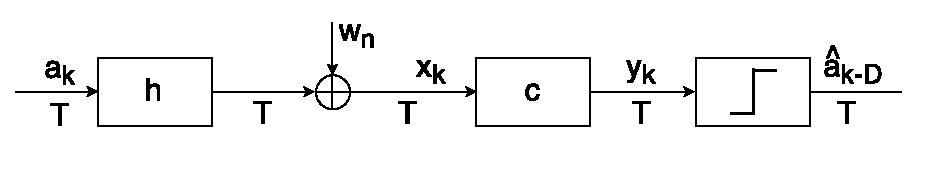
\includegraphics[width = 0.7\textwidth]{LE}
	\caption{LE filter}
	\label{fig:LE}
\end{figure}

\begin{figure}[h!]
	\centering
	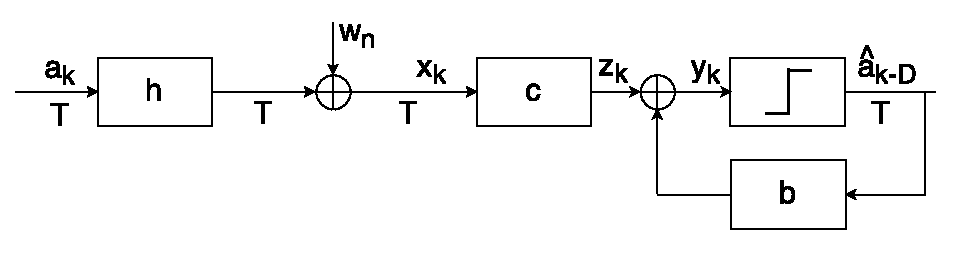
\includegraphics[width=0.7\textwidth]{DFE}
	\caption{DFE filter}
	\label{fig:DFE}
\end{figure}


% Considerazioni su Viterbi, Kd, grafico della distribuzione
\subsection*{Viterbi algorithm}

The Viterbi algorithm was implemented as a MATLAB function that performs the maximum likelihood detection using the whole message, including the known PN preamble for channel estimation, with initial conditions set to zero. Therefore, the initial conditions for the detection of the actual data (i.e. without the preamble) are given by the final symbols of the training sequence, which also has the function of training the Viterbi algorithm. The parameters $L_1 = 0$ and $L_2 = 4$ are set equal to $N_1$ and $N_2$ from problem 1.

The state of the FSM associated with the algorithm at time $k$ is as in \cite{bc}:
\begin{equation}
	\mathbf{s}_k = (a_{k+L1}, \ldots, a_{k-L_2+1}) = (a_k, \ldots, a_{k-3}), \quad k=0...K-1,
	\label{eq:state}
\end{equation}
where $K$ is the length of the input sequence, therefore the number of states is $N_S = M ^ {L_1 + L_2} = 4^4 = 256$. We associate each symbol of the QPSK constellation to an index $\alpha = 0,\ldots,3$ (the rule is arbitrary and it does not affect the result), so that a symbol $a_k$ at time $k$ is mapped to the corresponding index $\alpha_k$. The internal representation of the state is an integer in base $M$, with the most recent symbol in the least significant position, such that the state $\mathbf{s}_k$ is mapped to the integer
\begin{equation}
s_k = \sum_{i=0}^{L_1+L_2-1} M^i \alpha_{k+L_1-i} = \sum_{i=0}^{3} M^i \alpha_{k-i}.
\end{equation}
At time $k$, given the state $\mathbf{s}_{k-1}$ represented by $s_{k-1}$, and assuming the new symbol is $a_k$, the new state index is obtained by setting to 0 the two most significant bits (corresponding to the oldest symbol), shifting left by 2 bits and then adding the index of the new symbol in the two least significant bits:
\begin{equation}
s_k = \left[ (s_{k-1}) \lmod{M^{L_1+L_2-1}} \right] M + \alpha_k = 4 \, \left[ (s_{k-1})\lmod{64} \right] + \alpha_k.
\label{eq:newstateexpression}\end{equation}

In our implementation, we check all possible transitions by cycling through all state indices $s_{k-1}$ and considering for each of them the $M=4$ new possible symbols. Let the sequence of new state indices $s_k$ defined with this double iteration be $\{ s_k^{(i)} \}_{i=0,\ldots,MN_S-1}$, that has length $MN_S = M^{L_1+L_2+1} = 1024$.  Then, we have
\begin{equation}
s_k^{(i)} = i \mod N_S,
\end{equation}
hence a simple way of defining the new state indices is initializing a counter to 0 and incrementing it at every iteration of the inner loop, setting it again to 0 every time it reaches the value $N_S$. In fact, let us examine the first $N_S$ iterations, that correspond to $\frac{N_S}{M}$ iterations of the outer loop, in which the state indices $s_{k-1} = 0,\ldots,\frac{N_S}{M}-1$ are considered. Then, the first term of \eqref{eq:newstateexpression} takes the sequence of values
\begin{equation}
0,\,M,\,2M,\,\ldots,\,\left(\frac{N_S}{M}-1\right)M,
\end{equation}
that only has multiples of $M$. For each of them, the inner loop adds a term that takes values $0,\ldots,M-1$. Hence, the overall sequence cycles through all integers from $0$ to $N_S-1$, and the same reasoning applies for iterations $N_S +1$ to $MN_S$ -- the only difference is in the 2 most significant bits of $s_{k-1}$ that are discarded by the modulo operation. Since in our case $M=4$, this wrapping of the sequence happens 4 times.

Using the notation of \cite{bc}, we define $u_k$ as the desired received signal that carries information, that is the convolution of the sent symbol with the impulse response of the channel:
\begin{equation}
u_k = \sum_{n=-L_1}^{L_2} h_n a_{k-n} = \sum_{n=0}^{4} h_n a_{k-n}.
\label{eq:ukdefinition}\end{equation}
We observe that, given a fixed impulse response of the channel, $u_k$ only depends on the symbols $a_{k-4},\ldots, a_k$, which equivalent to say that it is a function of the current and the previous state, or of the current symbol and the previous state, i.e.
\begin{equation}
u_k = f_1(\mathbf{s}_{k-1}, \mathbf{s}_k) = f_2(\mathbf{s}_{k-1}, a_k) = f(s_{k-1}, \alpha_k),
\end{equation}
where $f$ has support $\{0,\ldots,N_S-1\} \times \{0,\ldots,M-1\}$. In the initialization phase of the algorithm, we build a $N_S \times M$ matrix, according to \eqref{eq:ukdefinition}, to be used during execution as a lookup table to determine the value of $u_k$ given the previous state and the current assumed received symbol. Note that in the first iterations $u_k$ depends on the initial conditions on the sequence $\{a_i\}$, that in our case were set to zero, therefore the lookup table is formally inaccurate. However, this transient error disappears completely before the end of the training sequence, thus the detection of the actual data is formally and practically correct.

At time $k$, for each possible previous state $\mathbf{s}_{k-1}$, the cost metric
\begin{equation}
\Gamma_k = \sum_{i=0}^k |\rho_i - u_i|^2
\end{equation}
is computed recursively as
\begin{equation}
\Gamma_k = \Gamma_{k-1} + |\rho_k - u_k|^2,
\end{equation}
where $\rho_k$ is the observed sample at time $k$ and $\Gamma_{k-1}$ is the cost metric of the assumed state $\mathbf{s}_{k-1}$. The 4 possible values of $u_k$ are given by row $s_{k-1}$ of the lookup table, yielding 4 different values of $\Gamma_k$ according to the new symbol $a_k$. These 4 values of $\Gamma_k$ are always associated to different states $\mathbf{s}_k$, and each of the new states $\mathbf{s}_k$ has 4 values of $\Gamma_k$ depending on the transition the system used to get to this state. Instead of storing all $MN_S$ values of $\Gamma_k$, we only keep track of the lowest $\Gamma_k$ for each new state $\mathbf{s}_k$, and we record the predecessor $\mathbf{s}_{k-1}$ (by means of its index $s_{k-1}$) that yielded the lowest cost. Finally, we make the decision on the oldest symbol of the survivor sequences according to the cost metric $\Gamma_k$, and we store the new survivor sequences with the respective costs.
%TODO use notation \Gamma(\mathbf{s}_k) ?

The survivor sequences at time $k$ are stored as symbols of the constellation, i.e. $a_{k-K_d} \ldots,a_{k-1}$, and the symbol $a_{k-K_d}$ is decided at the end of the $k$-th iteration. Therefore the Viterbi algorithm has a finite memory, that is the length $K_d$ of the trellis diagram, also known as trellis depth. It may happen that at time $k$ the symbols $a_{k-K_d}$ of all survivor sequences are the same, which means that the $(k-K_d)$-th symbol, and the previous ones, are already fixed: there is no point in keeping them in the survivor sequences, so we discard them and store the correct symbol in the vector of decided data. On the other hand, if the symbols $a_{k-K_d}$ of the survivor sequences are different then we are deciding based on the path metric up until $k$ (that is $\Gamma_k$), whereas we should decide the whole sequence according to the path metric computed on the whole message. This is an approximation that can in general yield some inaccuracies in the detection. The goal is to minimize $K_d$ for efficiency, without affecting too much the results.

We run 16 simulations of the transmission of 3 ML sequences with length $2^{20} - 1$ over our channel, with the setup used for all experiments of problem 2, and a Viterbi detector with $K_d = 80$. At each iteration (starting after the transient $K_d$), the modified Viterbi detector checks which is the minimum value of $K_d$ that would yield no premature decision. All survivor sequences contain the same symbols from a certain column backwards, and that column is given by the minimum $K_d$ needed.

Finally, we average the results of all experiments to obtain a complementary CDF for the minimum $K_d$. If the resulting complementary CDF is $y$ for a certain value of $K_d$, then for that $K_d$ the number of iterations in which the decision on the oldest symbol is actually made among different symbols is $y$ times the total number of iterations (minus the number of iterations of the transient, during which the survivor sequence is filled for the first time). In those cases, the symbol that belongs to the most likely sequence is chosen, which might turn out to be a suboptimal decision. The number of times we make this approximation on the Viterbi algorithm is $y$ times the length of the sequence.

The complementary CDF we get is shown in Fig.~\ref{fig:Kd_min_estimation}, from which we chose $K_d = 28$, that yields a probability of at most $7\cdot 10^{-7}$ that the first column of the matrix has different symbols. Therefore, the probability of making a wrong choice due to this approximation cannot be more than $7\cdot 10^{-7}$, which is reasonable unless we are trying to measure SNR's on that order of magnitude.

\begin{figure}
 \centering
 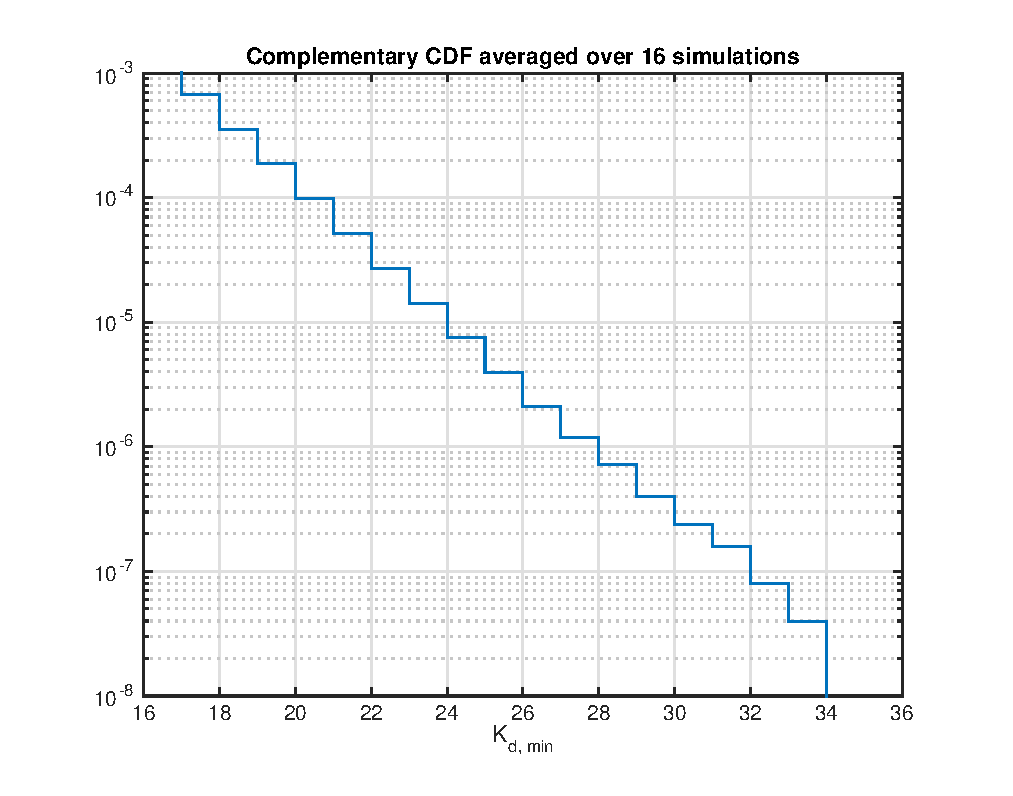
\includegraphics[width = 0.75\textwidth]{Kd_min_estimation}
 \caption{Complementary empirical CDF of $K_{d,\mathrm{min}}$ for the choice of $K_d$, over 16 independent simulations.}
 \label{fig:Kd_min_estimation}
\end{figure}


%%% Considerazioni su FBA (dettagli implementativi)
% - Considerazioni sull'occupazione di memoria e sulla velocità in riferimento al Viterbi
\subsection*{Max-Log-MAP}
Using the maximum a posteriori probability (MAP) criterion, the decision upon a received symbol is performed according to the expression:
\begin{equation}
	\hat{\boldsymbol{a}} = \argmax_{\boldsymbol{\alpha}} P[\boldsymbol{a} = \boldsymbol{\alpha} | \boldsymbol{z} = \boldsymbol{\rho}]
\end{equation}
where $\hat{\boldsymbol{a}}$ is the sequence of the detected symbols, $\boldsymbol{a}$ is that of the sent symbols, $\boldsymbol{\alpha}$ are the values of the sent symbols, $z$ is the sequence of the received symbols and $\boldsymbol{\rho}$ are the values of the received symbols.
If we introduce the \emph{likelihood function}
\begin{equation}
	\mathtt{L}_k(\beta) = P[a_{k+L_1} = \beta | \mathbf{z}_0^{K-1} = \boldsymbol{\rho}_0^{K-1}]
\end{equation}
the criterion becomes:
\begin{equation}
	\hat{a}_{k+L_1} = \argmax_{\beta \in \mathcal{A}} \mathtt{L}_k(\beta)
\end{equation}
In order to solve the problem of the likelihood function maximization, the FBA algorithm can be used. The algorithm performs the computation of four metrics, namely:
\begin{itemize}
	\item The Forward metric, $F_k(j)$
	\item The Backward metric, $B_k(j)$
	\item The State metric, $V_k(j)$
	\item The Likelihood function of the generic symbol,
	\begin{equation}
	 	\mathtt{L}_k(j) = \sum_{\substack{i = 1 \\ [\boldsymbol{\sigma}_i]_1 = \beta}}^{N_S} V_k(i) \quad \beta \in \mathcal{A}
	 \end{equation} 
\end{itemize}
where k is the variable associated with the symbol index and j is the state index, as defined in the Viterbi algorithm~\eqref{eq:state}.

Applying the logarithm to the above metrics yields the \emph{log-likelihood} function, whose expression is 
\begin{equation}
	\ell_k(\beta) = \ln \mathtt{L}_k(\beta) = \ln \sum_{\substack{i = 1 \\ [\boldsymbol{\sigma}_i]_1 = \beta}}^{N_S} e^{v_k(i)} \quad \beta \in \mathcal{A}
\end{equation}
where $v_k(i) = \ln V_k(i)$ is the logarithm of the state metric.

Using the logarithm the difference between the state metrics is enhanced, and as a result one term usually dominates within each time index $k$ in the sum above. Therefore, we can introduce the Max-Log-MAP criterion:
\begin{equation}
	\hat{a}_{k+L1} = \argmax_{\beta \in \mathcal{A}} \tilde{\ell}_k(\beta)
	\label{eq:decision}
\end{equation}
where the following approximation holds:
\begin{equation}
	\tilde{\ell}_k(\beta) = \max_{\substack{i \in [1, \dots, N_S] \\ [\boldsymbol{\sigma}_i]_1 = \beta}} v_k(i)
	\label{eq:likelihood}
\end{equation}

In our implementation we perform three main cycles in order to get all the metrics needed to compute $\tilde{\ell}$. 

The first cycle computes the channel transition metrics, storing them in a $M \times N_S \times K$ matrix where for a fixed time $k = 1, \dots, K$ the $M$ elements in the j-th column represent the transitions metrics from the state j. The metrics are computed using the following expression: 
\begin{equation}
	c_k(j|i) = - |\rho_k - u_k|^2
\end{equation}
Since the desired signal $u_k$ is just a function of the current and next state, its values are precomputed like in the Viterbi implementation~\eqref{eq:ukdefinition} and stored in a lookup table. $\rho_k$ represents the k-th sample of the received signal. For each time $k$, the $j$ index refers to the destination state, while the $i$ index refers to the starting state. Using matrix operations in MATLAB, we can fill the $c$ matrix by only cycling over time. For $k = K$ all values are set to 0.

The second cycle computes the Backward metric. A matrix of size $N_S \times K+1$ is created and initialized to zero. This also initializes the final, K-th state to the 0 value, since the final symbol that will be received is unknown (performance of the algorithm may be enhanced by transmitting a previously decided symbol, also known to the receiver). The algorithm cycles the symbol indices from $K-1$ to $0$, iterating over the states and updating their backward metric according to the following expression:
\begin{equation}
	\tilde{b}_k(i) = \max_{m \in [1, \dots, N_S]}[\tilde{b}_{k+1}(m) + c_{k+1}(m|i)] \quad i = 1, \dots, N_S
\end{equation}
At each time $k$, the indices $m$ of the states which are reachable from the current one are needed. These indices are computed using the expression $m = ((i-1) \lmod{M^{L1+L2-1}}) * M + j$, where $i$ is the current state and $j = 0, \dots, M-1$ is the index of the transition. On the other hand, the $c_{k+1}(m|i)$ coefficients are readily available as the i-th column of the channel transition metrics at time $k+1$.

The final cycle is used to compute the $\tilde{f}_k(j)$ metric for each state at each symbol index $k$. Since the State metric is $\tilde{v}_k(i) = \tilde{f}_k + \tilde{b}_k(i)$ for $i = 1, \dots, N_S$, there is no need to memorize $\tilde{f}_k(i)$ for every time index. A single iteration is performed in order to cover all the symbol indices from $0$ to $K-1$. For each $k$, another iteration over the $N_S$ states fills the vector of the forward metrics for all the states of the current $k$ index using the equation
\begin{equation}
	\tilde{f}_k(j) = \max_{\ell \in [1, \dots, N_S]} [\tilde{f}_{k-1}(\ell) + c_k(j|\ell)] \quad j = 1, \dots, N_S
\end{equation}
and the state metric is computed by adding this vector to the one memorized during the previous cycle, containing the backward metric. To get the channel transition metrics $c_k(j|\ell)$, the indices $\ell$ of the states that can reach the current one are necessary. These indices are computed according to the following expression: $\ell = \ceil{\frac{j}{M}} + r*M^{L1+L2-1}$, where $r = 0, \dots, M-1$. 
After computing the State metric $\tilde{v}_k(i) = \tilde{f}_k + \tilde{b}_k$ for $i = 1, \dots, N_S$, the likelihood function is obtained using~\eqref{eq:likelihood}: in order to decide which state metrics should be compared, we make use of a precomputed matrix of size $N_S \times M$ which contains the symbols associated to each state and pick only those states whose initial symbol is $\beta$. Finally, the decision is performed inside the same cycle according to~\eqref{eq:decision}, and the result is memorized in a vector.

Memory occupation for the Max-Log-MAP criterion is a concern. Since the Backward and channel transition matrices are memorized, their total memory occupation is of $M \times N_S \times K + N_S \times K$ memory cells. Computation times for the Max-Log-MAP have been more or less twice those of the Viterbi algorithm for sequences of the same length.
% TODO Refine this stuff above here

% Grafici del BER, sia per canale stimato che per canale vero, riportando il numero di bit per le simulazioni



\begin{thebibliography}{10}

\bibitem{bc}
Benvenuto, Cherubini, Algorithms for Communications Systems and their Applications, Wiley, 2004

\end{thebibliography}

\end{document}
